\documentclass[12pt, a4paper, oneside]{article}

\setlength{\parskip}{1ex plus 0.5ex minus 0.2ex}
\renewcommand{\baselinestretch}{1.1}

\usepackage[T1]{fontenc}
\usepackage{libertine}
\usepackage[english]{babel}
\usepackage[protrusion=true,expansion=true]{microtype}	
\usepackage{amsmath,amsfonts}
\usepackage[pdftex]{graphicx}	
\usepackage{url}
\usepackage{verbatim} 
\usepackage{hyperref}
\usepackage{cite}
\usepackage{mathtools}
\usepackage[colorinlistoftodos]{todonotes}
\usepackage[T1]{fontenc}
\usepackage{bookmark}
\usepackage{caption}
\usepackage{float}
\usepackage{enumitem}
\usepackage{textcomp}
\usepackage[sort,nameinlink]{cleveref}
\usepackage{amssymb}
\usepackage{xcolor}
\usepackage{booktabs}
\usepackage{multirow}
\usepackage{listings}
\usepackage{subcaption}
\usepackage{adjustbox}
\usepackage{algorithm}
\usepackage{algpseudocode}
\usepackage{lipsum}
\usepackage{geometry}
\usepackage{sectsty}
\usepackage{fancyhdr}
\usepackage{hyperref}

\geometry{
	a4paper,
	total={170mm,257mm},
	left=25mm,
	right=20mm,
	top=30mm,
	bottom=30mm
}

\hypersetup{colorlinks = true, allcolors=black}
%%% Custom sectioning
%\allsectionsfont{\normalfont\scshape}
%\allsectionsfont{\centering \normalfont\scshape}


%%% Custom headers/footers (fancyhdr package)
\pagestyle{fancyplain}
\fancyhead{}								% No page header
\fancyfoot[L]{}								% Empty 
\fancyfoot[C]{}								% Empty
\fancyfoot[R]{\thepage}							% Pagenumbering
\renewcommand{\headrulewidth}{0pt}					% Remove header underlines
\renewcommand{\footrulewidth}{0pt}					% Remove footer underlines
\setlength{\headheight}{13.6pt}


\lstset{breaklines}

%%%% Equation and float numbering
%\numberwithin{equation}{section}					% Equationnumbering: section.eq#
%\numberwithin{figure}{section}						% Figurenumbering: section.fig#
%\numberwithin{table}{section}						% Tablenumbering: section.tab#
\definecolor{MyDarkGreen}{rgb}{0.0,0.4,0.0}

\lstset{ % Use Perl in this example
	frame=single, % Single frame around code
	basicstyle=\small\ttfamily, % Use small true type font underlined and blue
	identifierstyle=, % Nothing special about identifiers                                         
	showstringspaces=false, % Don't put marks in string spaces
	tabsize=3, % 5 spaces per tab
	%
	% Put standard Perl functions not included in the default language here
	morekeywords={rand},
	%
	% Put Perl function parameters here
	morekeywords=[2]{on, off, interp},
	%
	% Put user defined functions here
	%	morekeywords=[3]{test},
	%
	numbers=left, % Line numbers on left
	firstnumber=1, % Line numbers start with line 1
	stepnumber=5 % Line numbers go in steps of 5
}


%%% Maketitle metadata
\newcommand{\horrule}[1]{\rule{\linewidth}{#1}} 	% Horizontal rule

\title{
	\pagestyle{empty}
	\usefont{OT1}{bch}{b}{n}
	\normalfont \large \textsc{Ho Chi Minh City University of Technology\\Faculty of Computer Science and Computer Engineering}\\ [48pt]
	
\includegraphics[scale=0.2]{bku}\\
	\vspace{25px}
	\horrule{0.5pt} \\[0.4cm]
	\huge -- Handwritten Digits Recognition System --
	Research Report
	\horrule{2pt} \\[0.5cm]
}
\author{
	\begin{tabular}{|c|l|c|}				\hline
		No. & \multicolumn{1}{c|}{Name} & Student ID \\ \hline
		1   & Nguyen Tien Anh           & 1752076    \\ \hline
		2   & Nguyen Minh Dang          & 1752170    \\ \hline
		3   & Tran Minh Hieu            & 1752199    \\ \hline
	\end{tabular}\\\\
	\textbf{Instructor:} Dr. Tran Ngoc Thinh
}
\date{\today}
\begin{document}
%--------------------------------------------- COVER PAGES ---------------------------------------------%
    \begin{titlepage}
	    \maketitle
	    \thispagestyle{empty}
    \end{titlepage}
    \newpage
    \pagenumbering{roman}

    \tableofcontents
    \newpage

    \listoffigures
    \newpage

    \pagenumbering{arabic}
    \setcounter{page}{1}
    \suppressfloats %No figures on first page
%--------------------------------------------- MAIN CONTENT ---------------------------------------------%
    \section{Introduction}
    	\subsection{Project}
    		The target is to implement a Handwritten Digits Recognition system using Machine learning based on the Zedboard FPGA development kit. The tool used to program the Zedboard is the Xilinx Vivado High-Level Synthesis (HLS). The project is built based on two programing languages: Python and C.
    	
    	\subsection{Zedboard}
    		ZedBoard™ is a complete development kit for designers using Xilinx Zynq®-7000 All Programmable SoC. The board provides various interfaces such as USB-JTAG Programming, USB OTG 2.0, USB-UART bridge, SD card and so on.  Combining a dual Corex-A9 Processing System (PS) with Programmable Logic (PL) cells, the Zedboard can be targeted  to use in many applications. 
    		
	    	\begin{figure}[tbh!]
	    		\begin{center}
	    			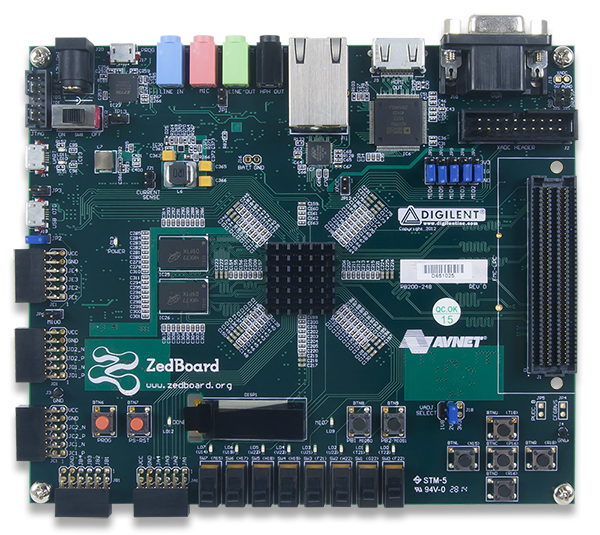
\includegraphics[scale=2.5]{zedboard.png}
	    			\caption{Zedboard}
	    			\label{fig:Zedboad}
	    		\end{center}
	    	\end{figure}
    	
    	\subsection{MNIST Database}
    		The dataset consists of 60000 digits for the training set and 10000 examples for the test set. Each digit have been size-normalized and centered in a fixed-size 28x28 pixel image. 
    			\begin{figure}[tbh!]
    				\begin{center}
    					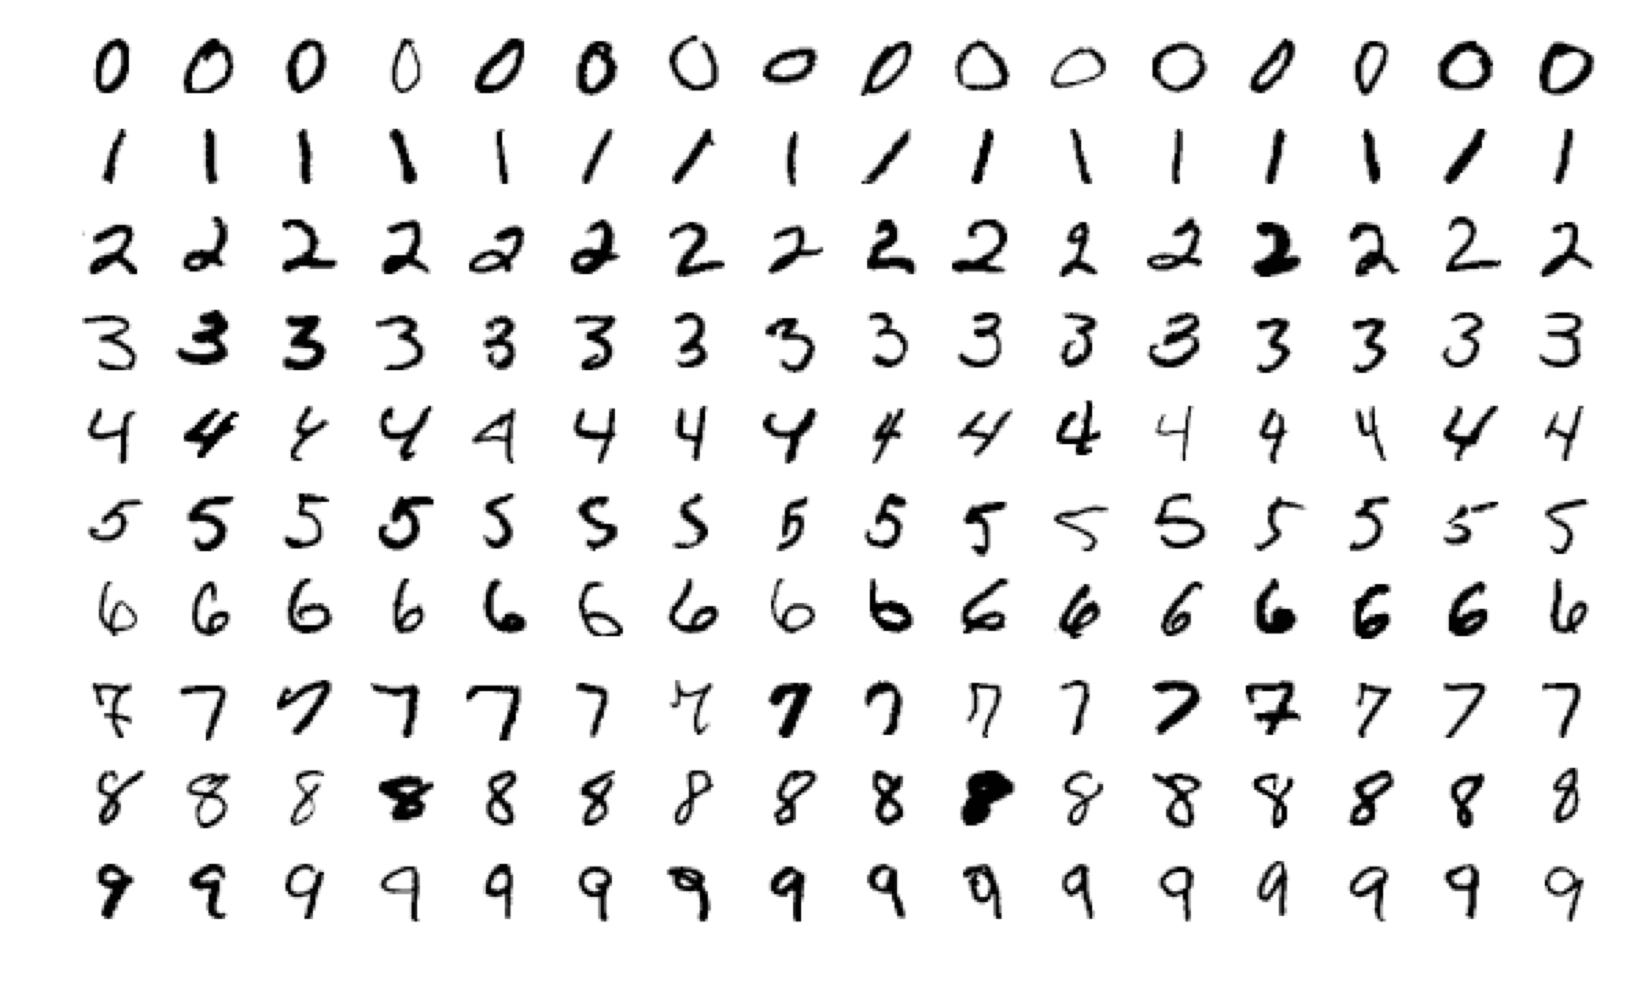
\includegraphics[scale=0.25]{MNIST.png}
    					\caption{MNIST Database}
    					\label{fig:MNIST Database}
    				\end{center}
    			\end{figure}
    		
    	\subsection{Algorithm}
    		In this project, the implementation of the system is based on Perceptron Learning Algorithm (PLA) - an algorithm for supervised learning of binary classifiers. A binary classifier is a function which can decide whether or not an input, represented by a vector of numbers, belongs to some specific class. 
    		
    \section{Methods}
    	\subsection{Pre-processing}
    		Before input to the system, an image goes through the 8-stage pre-processing procedure. 
    		\begin{figure}[H]
    			\begin{center}
    				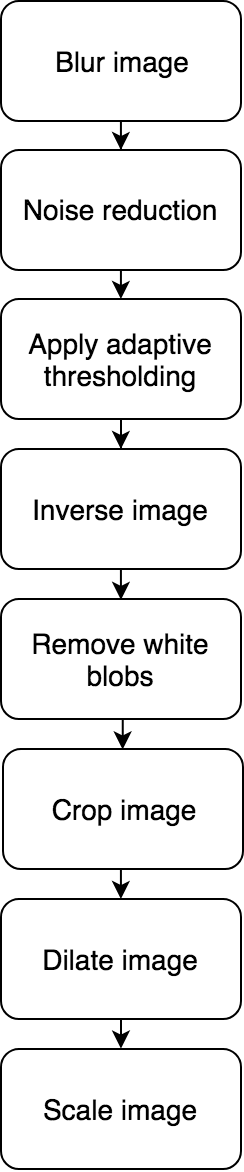
\includegraphics[scale=0.4]{preProcess.png}
    				\caption{Pre-processing}
    				\label{fig:Pre-processing}
    			\end{center}
    		\end{figure}
    
    	\subsection{Implement on Zedboard}
    		In this project, the Perceptron algorithm is programed on the Zedboard via Quad SPI Flash, which is a non-volatile memory Zedboard's Zynq chip looks at on every startup. If Quad SPI is flashed then the Zynq will program itself with the contents found in Quad SPI's Flash memory. A picture below indicates the set up of the Zedboard.
    		
    		\begin{figure}[tbh!]
    			\begin{center}
    				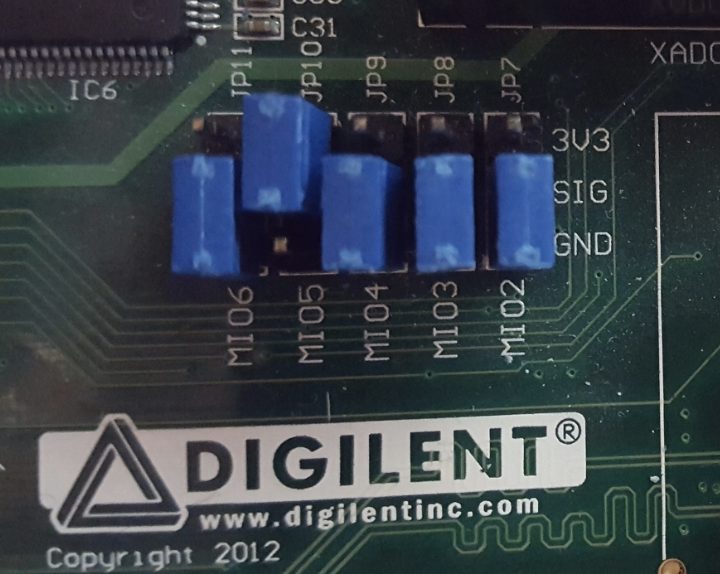
\includegraphics[scale=0.6]{QSPI.png}
    				\caption{Quad SPI Flash}
    				\label{fig:Quad SPI Flash}
    			\end{center}
    		\end{figure}
    		
    		In a high productivity design flow, the primary means of generating the core design IP is
    		through the use of C-based IP and High-Level Synthesis (HLS) of C code into RTL. The design flow for Vivado HLS is shown in the figure below. 
    		\begin{figure}[H]
    			\begin{center}
    				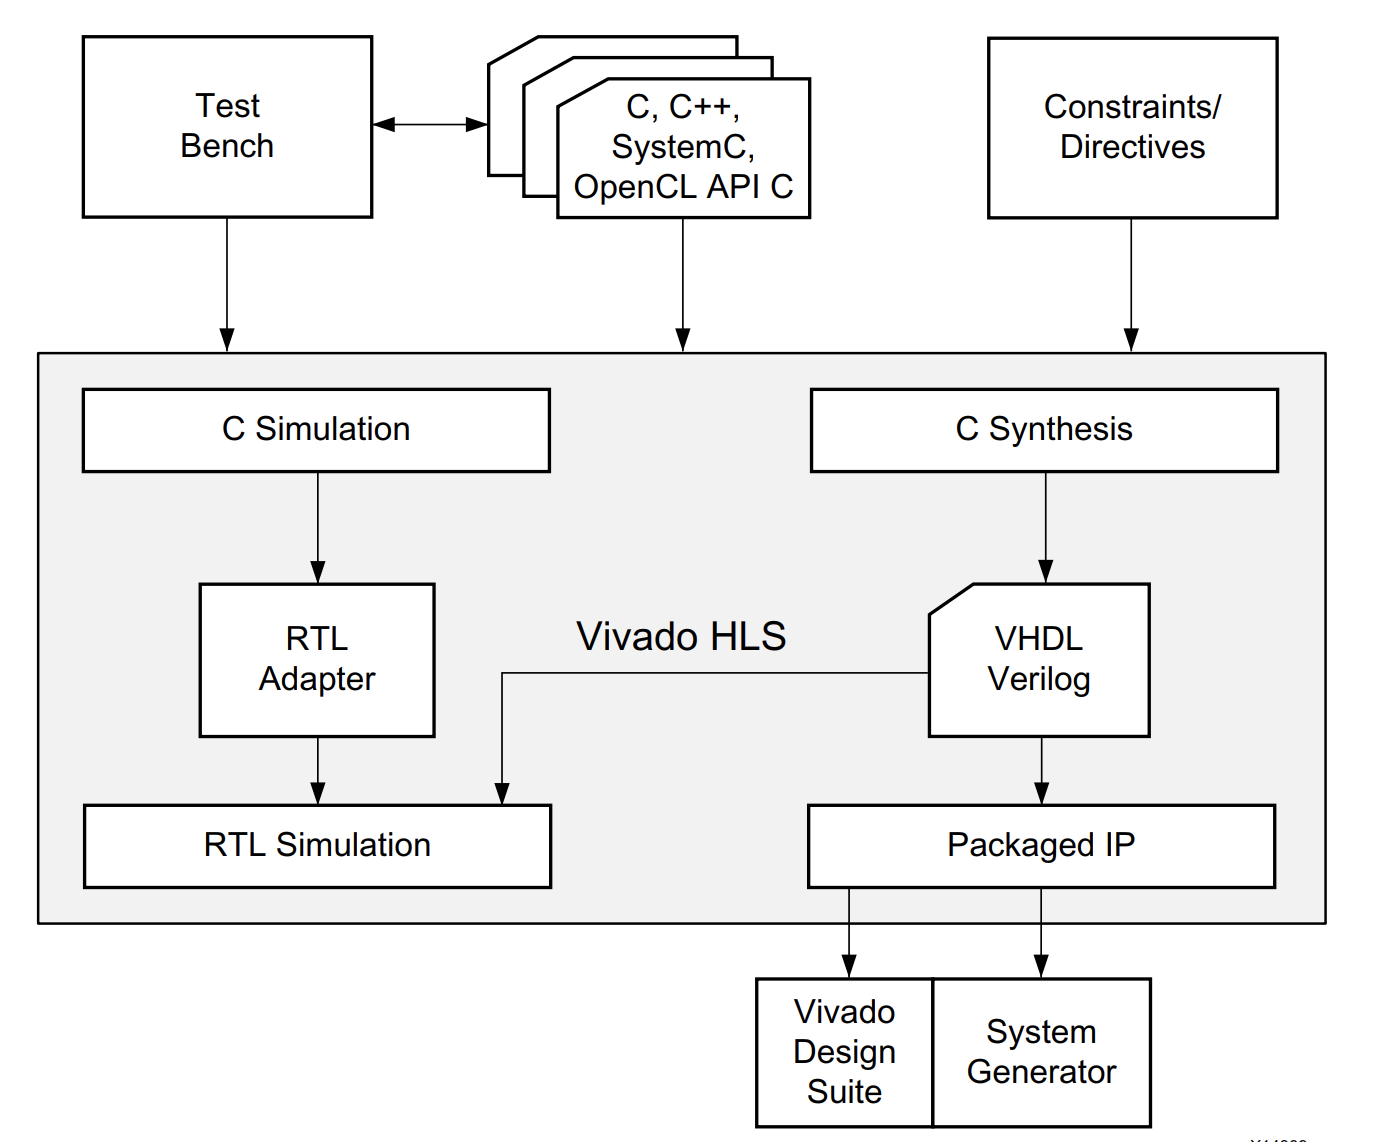
\includegraphics[scale=0.5]{HLS.png}
    				\caption{Vivado HLS deisgn flow}
    				\label{fig:Vivado HLS deisgn flow}
    			\end{center}
    		\end{figure}
    		
    \section{Results}
    	The source code of the project: \url{https://github.com/dangne/tkllHTR/}
    	
    \section{Discussion}
    
    
	\begin{thebibliography}{9}
    	\bibitem{zedboardwebsite} 
    	Zedboard
   		\\\texttt{http://zedboard.org//}
    		
	   	\bibitem{mistwebsite} 
	   	THE MNIST DATABASE of handwritten digits
	   	\\\texttt{http://yann.lecun.com/exdb/mnist/}
	   	
	   	\bibitem{perceptron} 
	   	Zedboard
	   	\\\texttt{https://machinelearningcoban.com/2017/01/21/perceptron/}
   \end{thebibliography}
	    
\end{document}
